\documentclass[11pt,a4paper]{article}
\usepackage[spanish,es-nodecimaldot]{babel}	% Utilizar español
\usepackage[utf8]{inputenc}					% Caracteres UTF-8
\usepackage{graphicx}						% Imagenes
\usepackage[hidelinks]{hyperref}			% Poner enlaces sin marcarlos en rojo
\usepackage{fancyhdr}						% Modificar encabezados y pies de pagina
\usepackage{float}							% Insertar figuras
\usepackage[textwidth=390pt]{geometry}		% Anchura de la pagina
\usepackage[nottoc]{tocbibind}				% Referencias (no incluir num pagina indice en Indice)
\usepackage{enumitem}						% Permitir enumerate con distintos simbolos
\usepackage[T1]{fontenc}					% Usar textsc en sections
\usepackage{amsmath}						% Símbolos matemáticos
\usepackage{listings}
\usepackage{algorithm}
\lstdefinelanguage{PDDL}
{
  sensitive=false,    % not case-sensitive
  morecomment=[l]{;}, % line comment
  alsoletter={:,-},   % consider extra characters
  morekeywords={
    define,domain,problem,not,and,or,when,forall,exists,either,
    :domain,:requirements,:types,:objects,:constants,
    :predicates,:action,:parameters,:precondition,:effect,
    :fluents,:primary-effect,:side-effect,:init,:goal,
    :strips,:adl,:equality,:typing,:conditional-effects,
    :negative-preconditions,:disjunctive-preconditions,
    :existential-preconditions,:universal-preconditions,:quantified-preconditions,
    :functions,assign,increase,decrease,scale-up,scale-down,
    :metric,minimize,maximize,
    :durative-actions,:duration-inequalities,:continuous-effects,
    :durative-action,:duration,:condition
  }
}
\lstdefinelanguage{JSHOP}
{
  sensitive=false,    % not case-sensitive
  morecomment=[l]{;}, % line comment
  alsoletter={:,-},   % consider extra characters
  morekeywords={
    defdomain,defproblem,not,and,or,imply,forall,assign,call,nil,
    :first,:sort-by,:immediate,:unordered,:operator,:method,:protection,:-
  }
}

% Comando para poner el nombre de la asignatura
\newcommand{\asignatura}{Técnicas de los Sistemas Inteligentes}
\newcommand{\autor}{Vladislav Nikolov Vasilev}

% Configuracion de encabezados y pies de pagina
\pagestyle{fancy}
\lhead{\autor{}}
\rhead{\asignatura{}}
\lfoot{Grado en Ingeniería Informática}
\cfoot{}
\rfoot{\thepage}
\renewcommand{\headrulewidth}{0.4pt}		% Linea cabeza de pagina
\renewcommand{\footrulewidth}{0.4pt}		% Linea pie de pagina

\begin{document}
\pagenumbering{gobble}

% Pagina de titulo
\begin{titlepage}

\begin{minipage}{\textwidth}

\centering

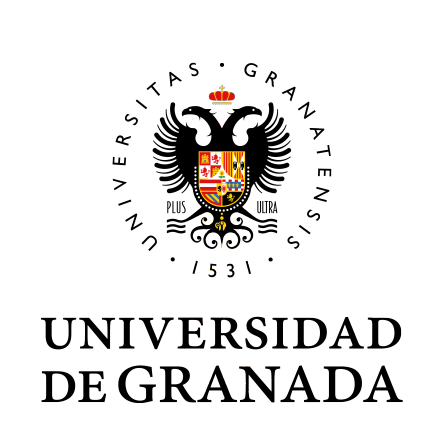
\includegraphics[scale=0.5]{img/ugr.png}\\

\textsc{\Large \asignatura{}\\[0.2cm]}
\textsc{GRADO EN INGENIERÍA INFORMÁTICA}\\[1cm]

\noindent\rule[-1ex]{\textwidth}{1pt}\\[1.5ex]
\textsc{{\Huge PRÁCTICA 2\\[0.5ex]}}
\textsc{{\Large Planificación Clásica\\}}
\noindent\rule[-1ex]{\textwidth}{2pt}\\[3.5ex]

\end{minipage}

\vspace{0.5cm}

\begin{minipage}{\textwidth}

\centering

\textbf{Autor}\\ {\autor{}}\\[2.5ex]
\textbf{Rama}\\ {Computación y Sistemas Inteligentes}\\[2.5ex]
\vspace{0.3cm}


\includegraphics[scale=0.3]{img/etsiit.jpeg}

\vspace{0.7cm}
\textsc{Escuela Técnica Superior de Ingenierías Informática y de Telecomunicación}\\
\vspace{1cm}
\textsc{Curso 2018-2019}
\end{minipage}
\end{titlepage}

\pagenumbering{arabic}
\tableofcontents
\thispagestyle{empty}				% No usar estilo en la pagina de indice

\newpage

\setlength{\parskip}{1em}

\section{Ejercicio 1}

A continuación se ofrece una descripción de las decisiones de diseño tomadas a la hora de realizar el ejercicio 1.

\subsection{Ejercicio 1.a}

Para representar los objetos del mundo se han utilizado tipos, y para dar un mayor nivel de abstracción, se han utilizado supertipos.
Por ejemplo, los distintos tipos de objetos (Manzana, Algoritmo, etc.) se han englobado bajo el supertipo \textit{items} para
poder facilitar referirse a cualquiera de ellos. Lo mismo pasa con los personajes, los cuáles han sido englobados bajo el supertipo
\textit{npc} para referirse a cualquiera de ellos. Y para todos los objetos que pueden ser puestos en alguna posición (jugador,
personaje al que dar un objeto y objeto) se han englobado bajo el supertipo \textit{locatable}. Todo esto se ha hecho, tal y como
se ha mencionado hace un momento, con el objetivo de facilitar la generalización al poder referirnos posteriormente a cualquier tipo
de personaje u objeto mediante un supertipo, en vez de tener que indicar el tipo concreto de un objeto.

A continuación se puede ver el dominio:

\begin{algorithm}[H]
\begin{lstlisting}[
  caption={Representación del dominio.},
  label={lst:pddlmove},
  language=PDDL]
(:types items npc Player - locatable
  	Oscar Manzana Algoritmo Oro Rosa - items
  	Princesa Principe Bruja Profesor Leonardo - npc
  	Player
  	zone
)
\end{lstlisting}
\end{algorithm}

\subsection{Ejercicio 1.b}

En este apartado se han representado los predicados básicos del dominio. Para representar las orientaciones del personaje y 
las posiciones relativas de dos zonas adyacentes (conexas), se han utilizado constantes que hacen referencia a cada uno de los
cuatro puntos cardinales (norte, sur, este y oeste). Se han elegido constantes debido a que son valores que no se van a instanciar
(no se van a crear variables de éstos ya que no tiene mucho sentido tenerlas), y como tal representan más un atributo o una propiedad
que un concepto u objeto.

En cuanto a los predicados, se han definido predicados para la orientación del jugador, las conexiones de zonas, las posiciones de
objetos, personajes y jugador (objetos con posición) y algunos predicados más que comentaremos.

Para la orientación del jugador, se utiliza el predicado \textbf{oriented}, el cuál indica qué jugador tiene qué orientación. Para
la localización de un objeto con posición se ha utilizado el predicado \textbf{at} que indica que el objeto con posición se encuentra
en una determinada zona. Se puede ver que aquí se ha utilizado una abstracción sobre un conjunto de conceptos para facilitar la
representación (como se indicó en el apartado anterior). Para representar las conexiones entre zonas se utiliza el predicado
\textbf{connected}, el cuál especifica que la primera zona está conectada zon la segunda zona mediante un punto cardinal (el cuál
reutiliza las constantes de orientación). Por ejemplo, si tuviésemos que desde una zona \textit{z1} se puede llegar a una zona
\textit{z2} la cuál se sitúa en el sur, tendríamos \textbf{(connected z1 S z2)}. Esto se ha hecho así para facilitar más adelante la
acción del giro, para poder comprobar más fácil si la orientación del jugador coincide con la de la zona a la que se quiere ir. El
predicado \textbf{emptyhand} indica que un determinado jugador tiene la mano vacía, y por tanto puede coger un objeto. Es importante
indicar esto, ya que si no, no habría forma de controlar si un jugador no tiene ya un objeto en la mano (recordemos que de momento
solo puede llevar un objeto). El predicado \textbf{taken} representa que un objeto (tipo \textit{item}) ha sido cogido por un jugador
determinado. El predicado \textbf{given} indica que un determinado objeto ha sido entregado a cualquier personaje. Esto se hace con el
objetivo de que el jugador no pueda quitarles a los personajes aquellos objetos que les hayan sido entregados. A parte de estos
predicados básicos, se tiene una función numérica \textbf{received} que indica cuántos objetos ha recibido un determinado personaje.
Cada vez que recibe uno, se incrementa el valor. Esto se ha hecho así para tener una especie de contador de objetos recibidos, el cuál
nos será útil más adelante. A continuación se pueden ver los predicados representados:

\begin{algorithm}[H]
\begin{lstlisting}[
  caption={Representación de predicados básicos.},
  label={lst:pddlmove},
  language=PDDL]
(:constants N S E W - orientation)
(:predicates
	(oriented ?p - Player ?o - orientation)
  	(at ?l - locatable ?z - zone)
  	(connected ?z1 - zone ?o - orientation ?z2 - zone)
  	(emptyhand ?p - Player)
  	(taken ?obj - items ?p - Player)
  	(given ?obj - items)
)
(:functions
  	(received ?n - npc)
)
\end{lstlisting}
\end{algorithm}

\subsection{Ejercicio 1.c}

Para este apartado se han creado acciones para girar al jugador tanto a la derecha como a la izquierda, desplazarse de una
zona a otra e interactuar con objetos y personajes.

Debido a que el código de las acciones es muy extenso, no se va a adjuntar en la memoria, si no que se va a comentar su funcionamiento
a algo nivel:

\begin{itemize}
	\item Para las acciones de giro, se comprueba la orientación del personaje, y según esta orientación se le asigna una nueva
	dependiendo del tipo de giro. Antes de esto, obviamente, se elimina la orientación antigua.
	\item Para moverse de una zona \textit{z1} a una zona \textit{z2}, se tiene que dar que el jugador se encuentre en la zona
	\textit{z1}, que las dos zonas estén conectadas y que el jugador esté orientado correctamente, ya que si no, tendrá que girar
	antes para orientarse correctamente. Al aplicar la acción, se cambia la posición del jugador y se elimina la anterior.
	\item Para coger un objeto se tiene que dar que el jugador tenga la mano vacía, ya que el jugador no puede coger más de un
	objeto simultáneamente (tendría que dejar el otro). Una vez que se aplica el objeto, el jugador deja de tener la mano vacía,
	el objeto no está en la zona en la que se encontraba y se indica que el objeto ha sido cogido por un determinado jugador.
	\item Para dejar un objeto, se tiene que dar que el jugador tenga cogido el objeto. Al dejarlo, se indica que el jugador ya no
	tiene cogido el objeto, que tiene la mano vacía y que el objeto se encuentra en la zona donde se encuentra actualmente el jugador.
	\item Para entregar un objeto, el jugador tiene que encontrarse en la misma zona que el personaje y tiene que tener cogido un
	objeto. Cuando se lo da, se indica que el jugador ya no tiene el objeto y que vuelve a tener la mano vacía. También se indica
	que el objeto se encuentra en la zona del personaje para intentar seguir una coherencia con la descripción del mundo, ya que
	al ser entregado no ``desaparece'', si no que el objeto se encuentra en una determinada zona del espacio, solo que ahora en
	posesión de un personaje. Para que no pueda volver a ser cogido y para representar que un personaje tiene posesión del objeto, se
	indica que el objeto ha sido entregado a un determinado personaje, y se incrementa el número de objetos que ha recibido dicho
	personaje. Ésto último, como se ha comentado antes, será muy significativo posteriormente.
\end{itemize}

\subsection{Ejercicio 1.d}

\section{Ejercicio 2}

A continuación se ofrece una descripción de las decisiones de diseño tomadas a la hora de realizar el ejercicio 2.

\section{Ejercicio 3}

A continuación se ofrece una descripción de las decisiones de diseño tomadas a la hora de realizar el ejercicio 3.

\section{Ejercicio 4}

A continuación se ofrece una descripción de las decisiones de diseño tomadas a la hora de realizar el ejercicio 4.

\section{Ejercicio 5}

A continuación se ofrece una descripción de las decisiones de diseño tomadas a la hora de realizar el ejercicio 5.

\section{Ejercicio 6}

A continuación se ofrece una descripción de las decisiones de diseño tomadas a la hora de realizar el ejercicio 6.

\section{Ejercicio 7}

A continuación se ofrece una descripción de las decisiones de diseño tomadas a la hora de realizar el ejercicio 7.

\end{document}

